\subsection{External Interface Requirements}

\subsubsection{User Interfaces}
\subsubsection{App Mockups}

 
\begin{multicols}{3}
\begin{figure}[H]

 \centering
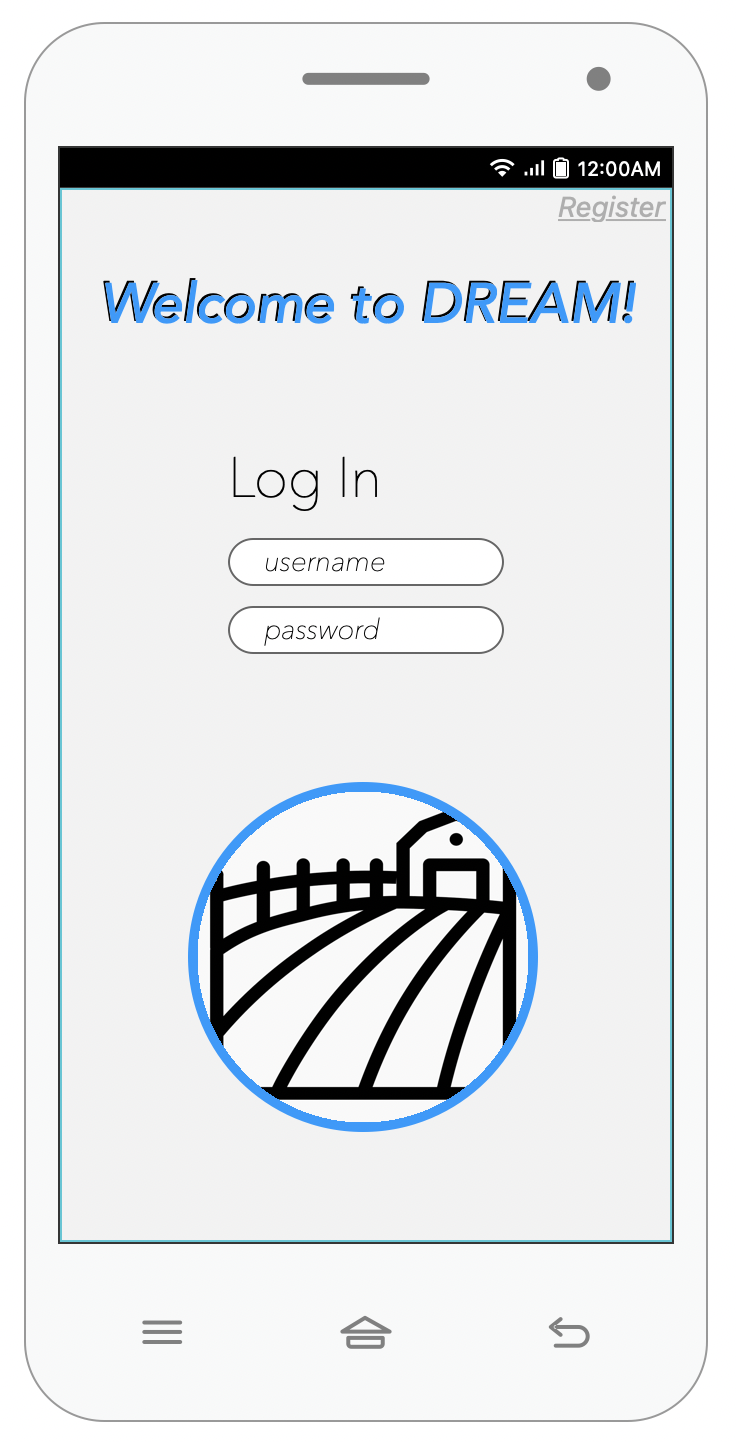
\includegraphics[scale=0.35]{../images_diagrams/mock_ups/login100.png}
 \caption{\label{fig:mock_login}Login Mock Up.}
 \end{figure}
 
 
\begin{figure}[H]
 \centering
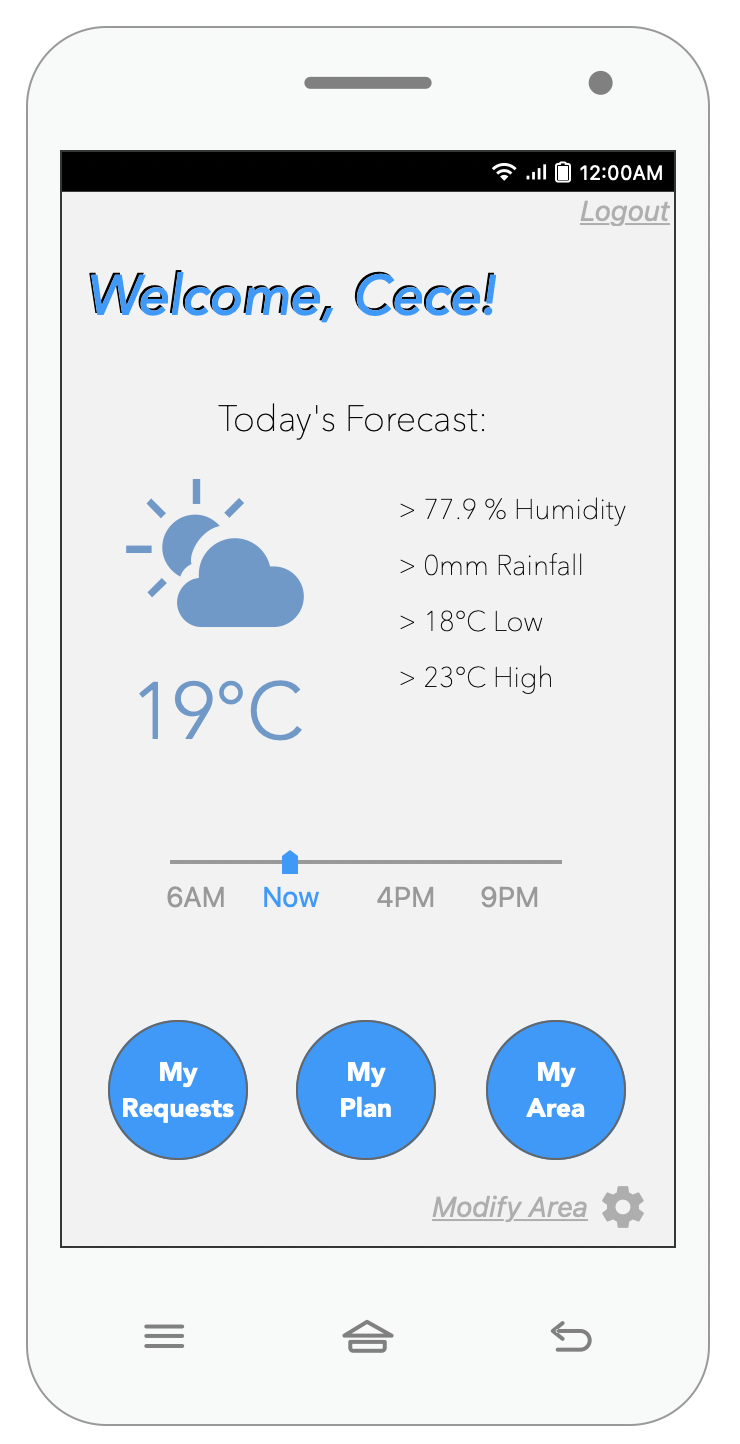
\includegraphics[scale=0.35]{../images_diagrams/mock_ups/welcomeagro100.png}
 \caption{\label{fig:mock_agronomist}Welcome Agronomist Mock Up.}
 \end{figure}
 
 
\begin{figure}[H]

 \centering
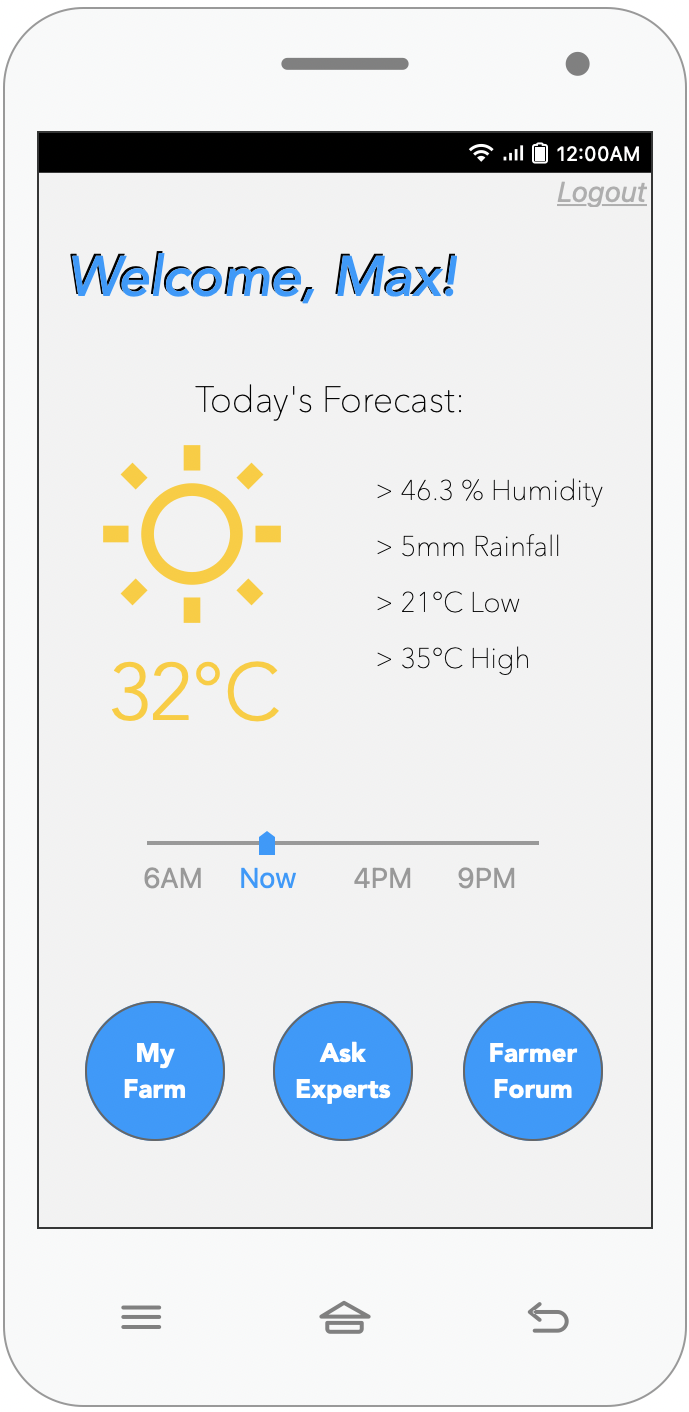
\includegraphics[scale=0.35]{../images_diagrams/mock_ups/welcomefarmer100.png}
\caption{\label{fig:mock_farmer}Welcome Farmer Mock Up.}
 \end{figure}
 
 
\begin{figure}[H]
 \centering
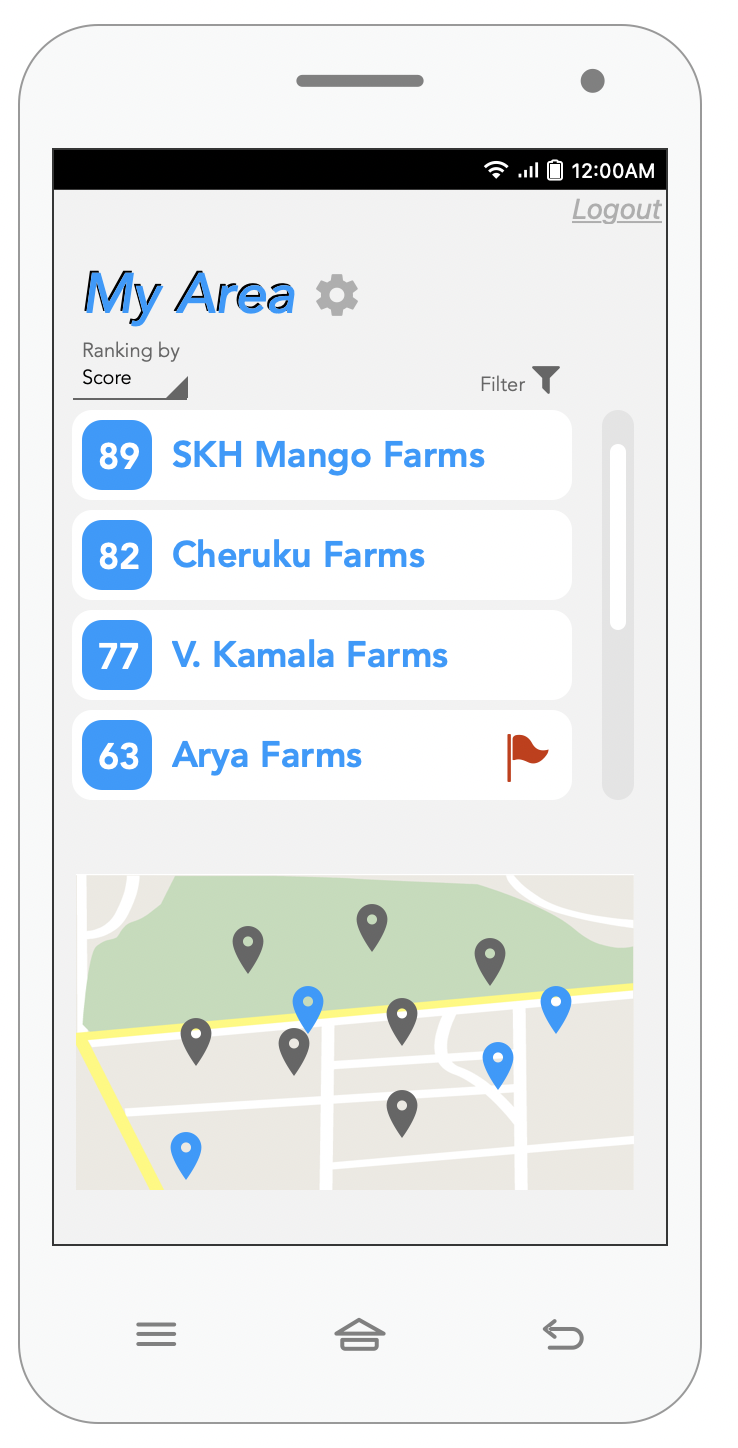
\includegraphics[scale=0.35]{../images_diagrams/mock_ups/myarea100.png}
\caption{\label{fig:mock_area}My Area Agronomist Mock Up.}
 \end{figure}
 
 
\begin{figure}[H]
 \centering
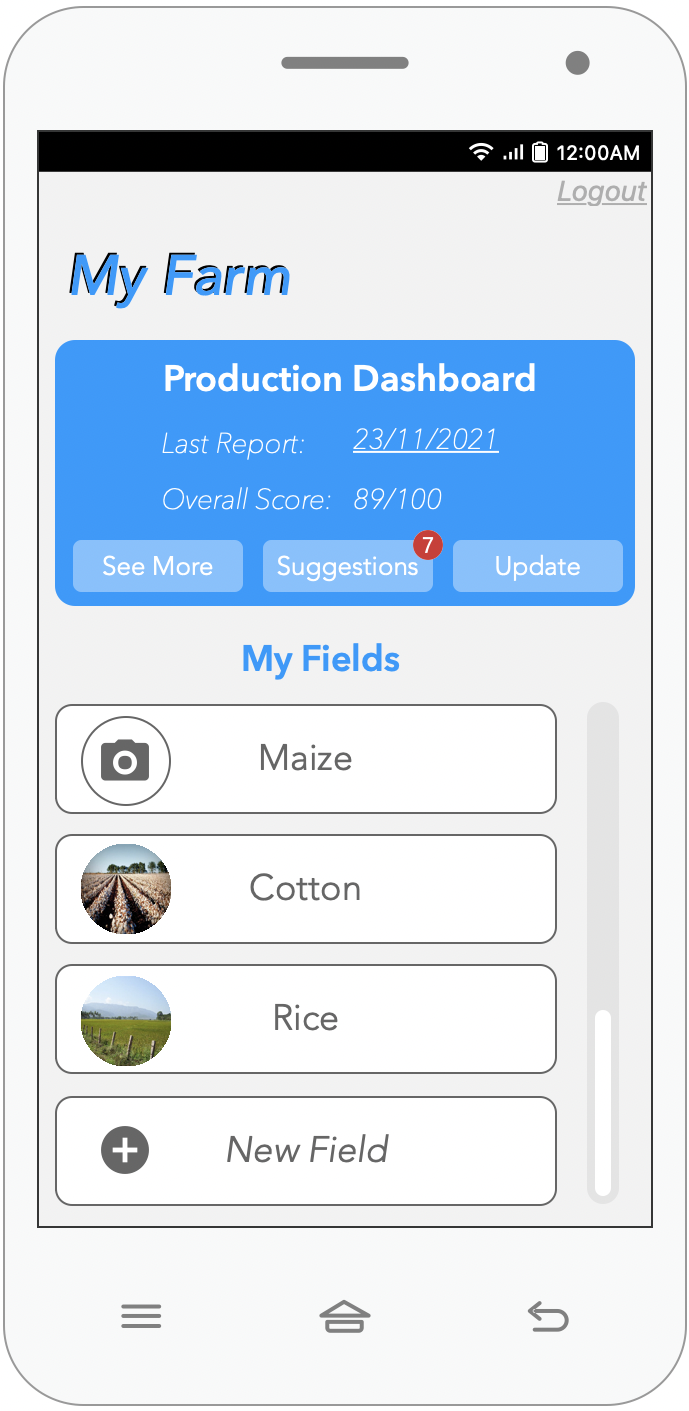
\includegraphics[scale=0.35]{../images_diagrams/mock_ups/myfarm100.png}
\caption{\label{fig:mock_farm}My Farm Mock Up.}
 \end{figure}
 
 
\begin{figure}[H]

 \centering
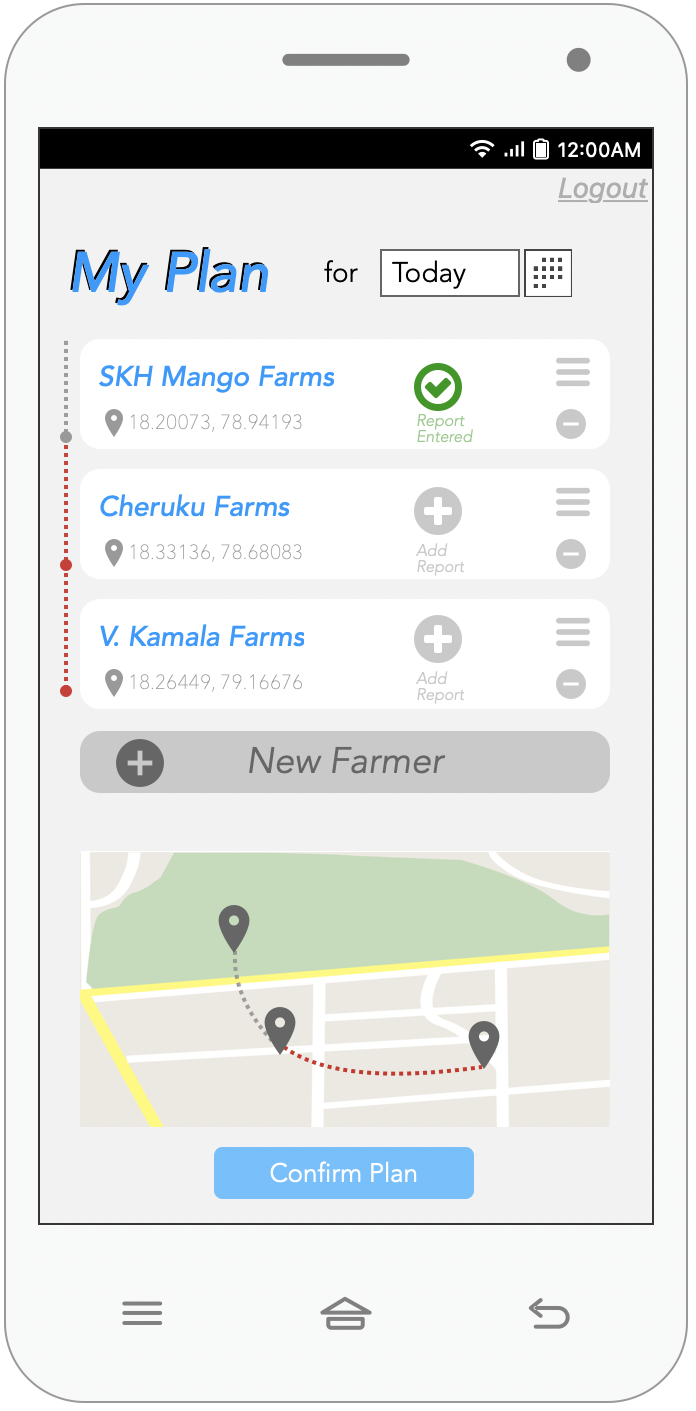
\includegraphics[scale=0.35]{../images_diagrams/mock_ups/myplan100.png}
\caption{\label{fig:mock_plan}My Plan Agronomist Mock Up.}
 \end{figure}
 
 
\begin{figure}[H]
 \centering
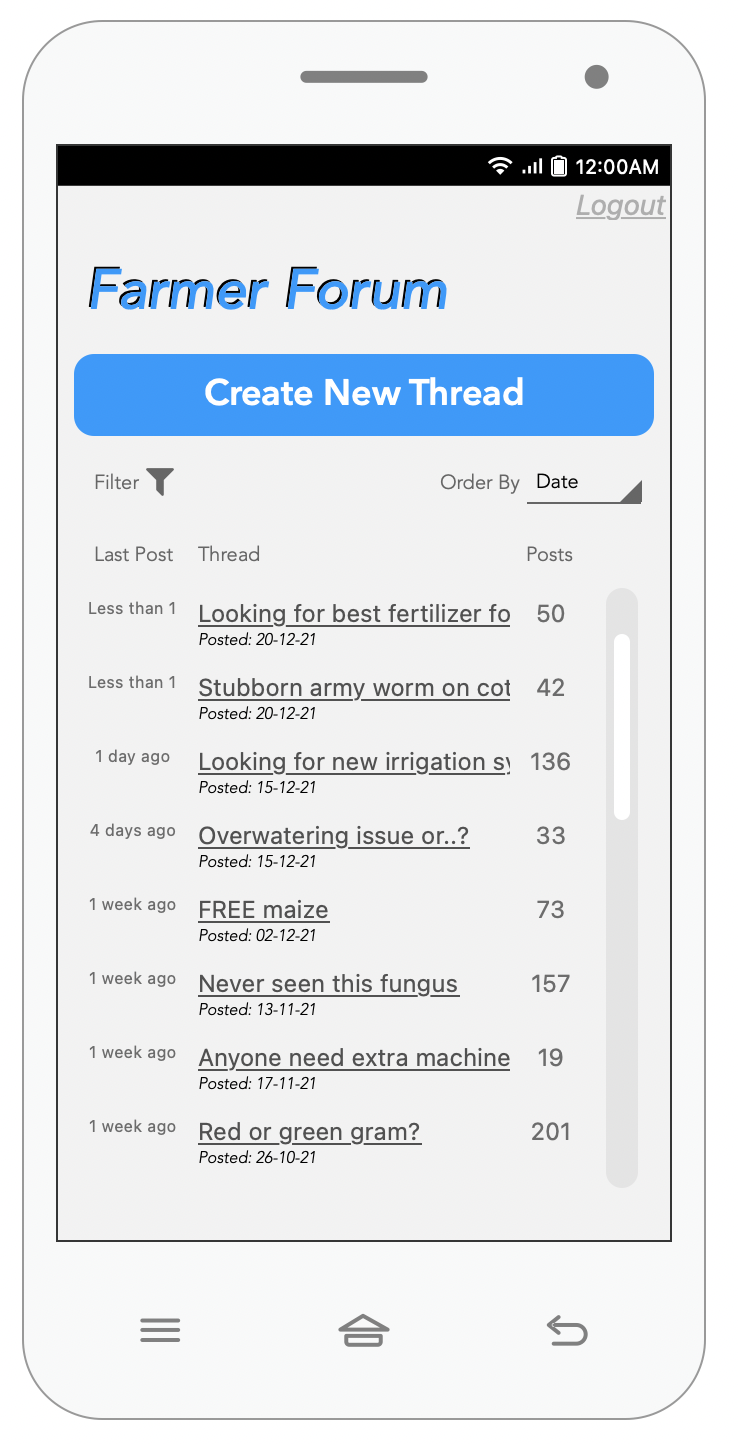
\includegraphics[scale=0.35]{../images_diagrams/mock_ups/farmerforum100.png}
\caption{\label{fig:mock_forum}Farmer Forum Mock Up.}
 \end{figure}
 
 
\begin{figure}[H]
 \centering
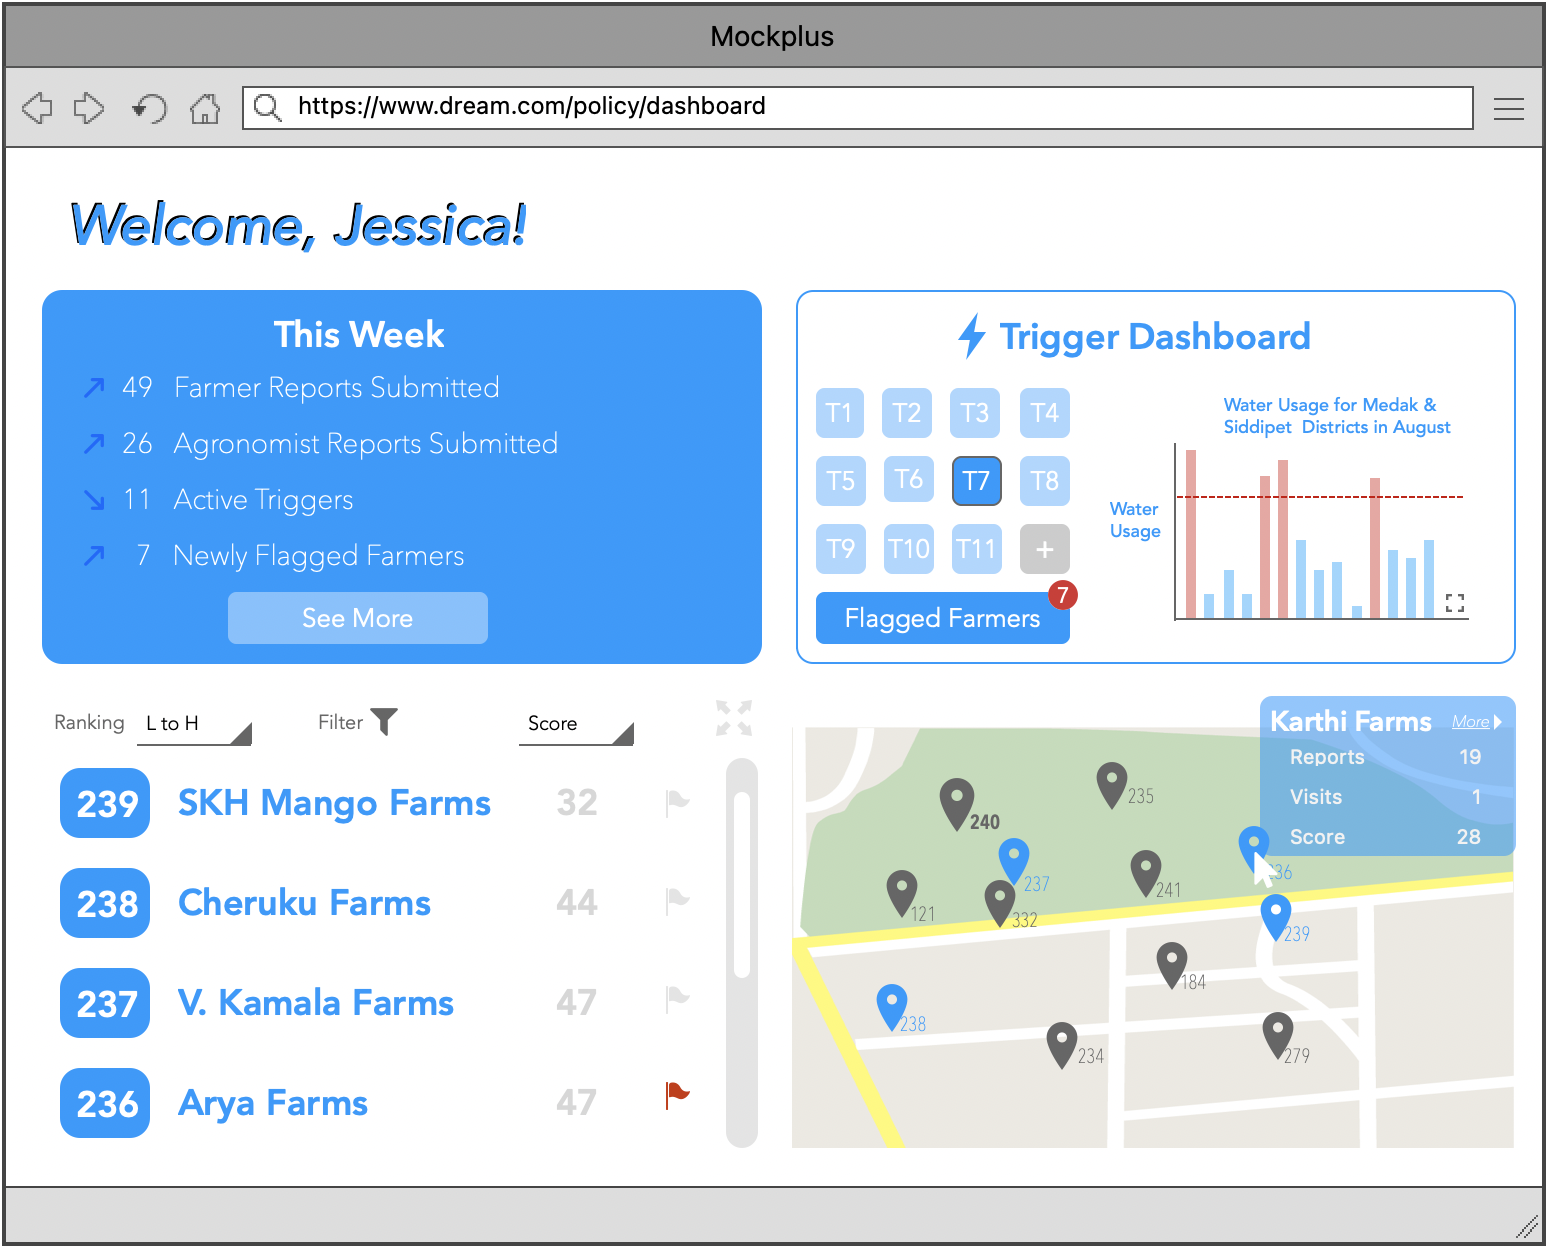
\includegraphics[scale=0.392]{../images_diagrams/mock_ups/policydash100.png}
 \caption{\label{fig:mock_polish}Policy Maker Dashboard Mock Up.}
 \end{figure}
 
 
\end{multicols}




\subsubsection{Hardware Interfaces}
\begin{flushleft}
All users will access the application with their own devices: mobile device, tablet device, or computer device.
The farmer's device needs the following in order to have full functionality of DREAM:
\begin{itemize}
\item Internet connection [required]: when the farmer is submitting their data while in their fields, their device will need to have an internet connection in order to access DREAM servers. In the event that an area has limited internet connection, the data will be temporarily saved locally on the user's device. The size of the data should be negligible with respect to the memory offered by commonly held devices.
\item Camera [optional]: farmers can submit pictures to aid their textual descriptions when posting in the discussion board or when messaging an agronomist. Although this is not required to use the application, it is highly recommended.
\item GPS sensor [optional]: farmers can either manually enter their location or allow the application to utilize the GPS sensor from their device.
\end{itemize}

The agronomist's device needs the following in order to have full functionality of DREAM:
\begin{itemize}
\item Internet connection [required]: when the agronomist is visiting farmers their device will need to have internet access in order for the agronomist to submit their reports to the DREAM servers throughout the day and to follow the navigation path calculated by DREAM.
\item GPS [optional]: since the agronomist will use a navigation plan generated by DREAM, sharing their GPS location is preferred for an optimal user experience. Without this device functionality, the agronomist will not be able to receive live turn-by-turn navigation guidance.
\end{itemize}

The policy maker's device needs the following in order to have full functionality of DREAM:
\begin{itemize}
\item Internet connection [required]: in order to access the rankings and evaluations of the farmers throughout the region, internet connection is required to access the DREAM servers.
\end{itemize}
\end{flushleft}

\subsubsection{Software Interfaces}
This product is accessible through a mobile-friendly application. Farmers will spend the majority of their time accessing the application through a mobile device; agronomists will access the application with both a mobile device and a computer device; policy makers will access the application almost exclusively with a computer device. Due to the mix of mobile and computer devices, the web application must be suitable for both interfaces.


\subsubsection{Communication Interfaces}
The mobile-friendly web application will communicate with DREAM servers over an internet connection.

\newpage
\subsection{Functional Requirements}

%Use this counter for the scenarios and command \addOne to print and increase at the same time
\newcounter{usecase_counter}
\setcounter{usecase_counter}{1}

The use case diagram in \textbf{Figure \ref{fig:usecase}} shows how the different actors expect to use the system. Each use case in the diagram can be further disseminated into other more specific use cases as described in the subsequent \textbf{Tables \ref{tab:farmerNewThread} - \ref{tab:policyUseViewRank}}.
\begin{figure}[htb!]\begin{flushleft}

\end{flushleft}
\centering
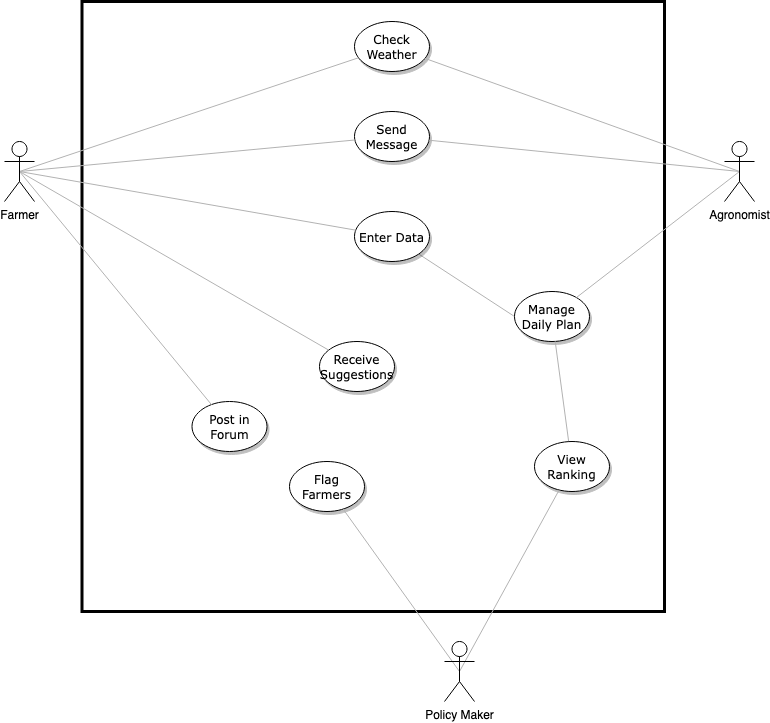
\includegraphics[scale=0.6]{../images_diagrams/usecasediagram.png}
\caption{\label{fig:usecase}Use case diagram.}
\end{figure}

%GENERICS USE CASES
% Use Case Table
\begin{center}
\renewcommand{\arraystretch}{1.25}
\begin{tabular}{|l|>{\raggedright\arraybackslash}m{12cm}|}
    \hline
    \textbf{Name} & User Registration\\
    \hline
   	\textbf{Actor} & Farmer, Agronomist, Policy Maker ???\\
    \hline
    \textbf{Entry Conditions} & \\
    \hline
    
    \textbf{Events Flow} & \begin{enumerate}
    			\item The user register on the site using his/her email.
    			\item The user gets an appointment to verify his/her identity.
    			\item The user profile is validated and obtains credentials.
	    		\end{enumerate}
    	\\
    \hline
    \textbf{Exit Conditions} & \begin{itemize}
    	\item The user has credentials of a validated account.
   		\end{itemize} \\
    \hline
\end{tabular}
\end{center}
% Use Case Table

\begin{center}
\begin{tabular}{|l|>{\raggedright\arraybackslash}m{12cm}|}

    \hline
    \textbf{Name} & \textit{User log-in}\\
    \hline
   	\textbf{Actor} & \textit{Farmer, Agronomist, Telangana's policy maker}\\
    \hline
    \textbf{Entry Conditions} & \textit{The user opens the application}\\
    \hline
    \textbf{Events Flow} & \textit{
    \begin{enumerate}
            \item The user press the "log-in" option on the screen
            \item The user inserts his credentials
            \item The user press the "log-in" button
            \item The user can then choose multiple farmers to visit that day from a list of recommended 					ones
     \end{enumerate}}\\
    \hline
    \textbf{Exit Conditions} & \textit{The system accepts the credentials  and the user is now able to perform actions inside the application}\\
    \hline
    \textbf{Exceptions} & \textit{
      \begin{itemize}
          \item The credentials are not valid, therefore the user will be asked to check her/his input
		\item The password is not correct so the user will be asked to insert the correct password. After three tries, the account is temporarily blocked and a reset mail is sent
        \end{itemize}
     }\\
    \hline
\end{tabular}
\end{center}
%FARMERS
\subsubsection{Farmer}
% Scenario Text
\begin{flushleft}
\textbf{Scenario \addOne{usecase_counter}:} 
Max is a farmer who cultivates some fields near his house in Telangana state. Max has been planting the same plant species over the last few years; he refrains from trying different plants because he is unfamiliar with the cultivation methods. Now, with more children and grandchildren to feed, he would like to change the crop with something more productive. Max learned about the DREAM initiative from a friend and, through the Association of Farmers, he received his credentials to log into the website.
Within minutes of accessing the site, he skimmed through the discussion forums and discovered that there are thousands of small farmers like him with the same doubts and fears. He learned which species are more productive and which fertilizer to use. Now he can feed his entire family and even sell some food to the local market.
\end{flushleft}
% Use Case Table
\begin{center}
\begin{tabular}{|l|>{\raggedright\arraybackslash}m{12cm}|}

    \hline
    \textbf{Name} & \textit{Create a thread in farmers' forum}\\
    \hline
   	\textbf{Actor} & \textit{Farmer}\\
    \hline
    \textbf{Entry Conditions} & \textit{The user uses valid credentials to log into the application}\\
    \hline
    \textbf{Events Flow} & \textit{
    		\begin{enumerate}
    			\item The user opens the forums section
    			\item The user clicks on "Create thread"
    			\item The user writes a valid title and message
    			\item The user clicks on "Publish"
    			\item The user can answer to messages published in his conversation
    		\end{enumerate}
    	}\\
    \hline
    \textbf{Exit Conditions} & \textit{The user closes the forum section or the entire application}\\
    \hline
    \textbf{Exceptions} & \textit{
    		\begin{itemize}
    			\item The server is not available
    		\end{itemize}
    	}\\
    \hline
\end{tabular}
\end{center}
% Use Case Table
\begin{center}
\renewcommand{\arraystretch}{1.25}
\begin{tabular}{|l|>{\raggedright\arraybackslash}m{12cm}|}

    \hline
    \textbf{Name} & Visit the discussion forum\\
    \hline
   	\textbf{Actor} & Farmer\\
    \hline
    \textbf{Entry Conditions} & The logs into the application with valid credentials.\\
    \hline
    \textbf{Events Flow} & 
    		\begin{enumerate}
    			\item The user opens the "Forums" section.
    			\item The user opens a thread and reads the conversation.
    			\item The user submits a post in an existing thread.
    		\end{enumerate}
    	\\
    \hline
    \textbf{Exit Conditions} & \begin{itemize}
    	\item The user exits the "Forum" section.
    	\item The user closes the entire application.\end{itemize}\\
    \hline
    \textbf{Exceptions} & 
    		\begin{itemize}
    			\item The server is not available.
    			\item There are no existing threads.
    		\end{itemize}
    	\\
    \hline
\end{tabular}
\end{center}
% Scenario Text
\begin{flushleft}
\textbf{Scenario \addOne{usecase_counter}:} 
Caroline has a big farm in Telangana state with 50 hectares of land and different varieties of plants. Last year, during the monsoon season, her fields were flooded, and almost no plants survived. In addition, this summer, the hot temperature killed some other species.
After consulting an expert, she decided to join the DREAM initiative to ask for direct support from agronomists and to obtain some incentives from the central government.
Next year she will plant more resilient crops and take some precautions against flooding.
\end{flushleft}
% Use Case Table
\begin{center}
\begin{tabular}{|l|>{\raggedright\arraybackslash}m{12cm}|}

    \hline
    \textbf{Name} & \textit{Asking advice to agronomists}\\
    \hline
   	\textbf{Actor} & \textit{Farmer}\\
    \hline
    \textbf{Entry Conditions} & \textit{The user uses valid credentials to log into the application}\\
    \hline
    
    \textbf{Events Flow} & \textit{
    		\begin{enumerate}
    			\item The user opens the "Ask to experts" section
    			\item The user selects the assigned agronomist
    			\item The user writes a short request and submit it
    			\item After receiving a notification, The user can see the answer
    			\item Eventually, The user can continue the conversation asking further questions
    		\end{enumerate}
    	}\\
    \hline
    \textbf{Exit Conditions} & \textit{The conversation is closed by either the farmer or the agronomist}\\
    \hline
    \textbf{Exceptions} & \textit{
    		\begin{itemize}
    		    	\item The server is not available
    			\item The agronomist doesn't answer to the message
    		\end{itemize}
    }\\
    \hline
\end{tabular}
\end{center}
% Use Case Table
\begin{table}[hbt!]
\centering
\caption{\label{tab:addOne{table_counter}}Farmer use case related to Scenario 2.}
\renewcommand{\arraystretch}{1.25}
\begin{tabular}{|l|>{\raggedright\arraybackslash}m{12cm}|}

    \hline
    \textbf{Name} & Upload information about production\\
    \hline
   	\textbf{Actor} & Farmer\\
    \hline
    \textbf{Entry Conditions} & The user logs into the application with valid credentials and has new data to upload.\\
    \hline
    
    \textbf{Events Flow} & 
    		\begin{enumerate}
    			\item The user opens the "My Production" section.
    			\item The user clicks on the "Update Production Data" button.
    			\item The user selects a field to update from a list of fields.
    			\item The user adds the desired information.
    			\item The user clicks on the "Submit" button.
    		\end{enumerate}
    	\\
    \hline
    \textbf{Exit Conditions} & The user submits the information.\\
    \hline
    \textbf{Exceptions} & 
    		\begin{itemize}
    			\item The server is not available.
    			\item The provided information is not valid.
    			\item Some required information is left empty.
    		\end{itemize}
    \\
    \hline
\end{tabular}
\end{table}

% Use Case Table
\begin{table}[hbt!]
\centering
\caption{\label{table:addOne{table_counter}}Farmer use case.}
\renewcommand{\arraystretch}{1.25}
\begin{tabular}{|l|>{\raggedright\arraybackslash}m{12cm}|}

    \hline
    \textbf{Name} & Add field location with GPS\\
    \hline
   	\textbf{Actor} & Farmer\\
    \hline
    \textbf{Entry Conditions} & The user logs into the application with valid credentials and is physically in the field.\\
    \hline
    \textbf{Events Flow} & 
    		\begin{enumerate}
    			\item The user opens the "My Farm" section.
    			\item The user clicks on the "Add New Field" button.
    			\item The user is prompted to allow the application to use their GPS location.
    			\item The user clicks on the "Allow" button, allowing the application to locate them using GPS.
    			\item The user adds information about the size of the field, crop currently planted, the fertilizer in use, and any other information they deem relevant.
    			\item The user clicks on the "Submit" button.
    		\end{enumerate}
    	\\
    \hline
    \textbf{Exit Conditions} & The user submits the information about the new field.\\
    \hline
    \textbf{Exceptions} & 
    		\begin{itemize}
    			\item The server is not available.
    			\item The application is not able to use the GPS.
    			\item The user doesn't allow the application to use GPS.
    			\item The provided information is not valid.
    			\item Some required information is left empty.
    		\end{itemize}
    \\
    \hline
\end{tabular}
\end{table}
% Use Case Table
\begin{center}
\renewcommand{\arraystretch}{1.25}
\begin{tabular}{|l|>{\raggedright\arraybackslash}m{12cm}|}
    \hline
    \textbf{Name} & Access weather forecast data\\
    \hline
   	\textbf{Actor} & Farmer\\
    \hline
    \textbf{Entry Conditions} & The user logs into the application with valid credentials and has at least one field registered with the application.\\
    \hline
    
    \textbf{Events Flow} & \begin{enumerate}
    			\item The user opens the "My Farm" section.
    			\item The user clicks on the "Weather" tab.
    			\item The user selects a field from a list of fields.
    			\item The user can see the weather associated with the location for the selected field.
	    		\end{enumerate}
    	\\
    \hline
    \textbf{Exit Conditions} & \begin{itemize}
    	\item The user closes the weather section.
    	\item The user navigates "Back" to the list of fields.
   		\item The user closes the entire application.
   		\end{itemize} \\
    \hline
    \textbf{Exceptions} &
    		\begin{itemize}
    			\item The server is not available.
    		\end{itemize}
    \\
    \hline
\end{tabular}
\end{center}


%AGRONOMISTS
\subsubsection{Agronomist}
%before: emails for help, data, now can consult

% Scenario Text
\begin{flushleft}
\textbf{Scenario \addOne{usecase_counter}:} 
Schmidt is an agronomist. His job is based on knowing farmers' information and helping them to improve and solve problems. Before installing DREAM he was receiving various emails from farmers. All the emails contained important information about them and help or suggestion requests. He then needed to combine the content from the emails with the information he provided about latest visits of their farm. Sometimes data were not in the same format and not standardized; this slowed his work. Now with DREAM he can easily inspect all of the data in the same place from the convenience of his device. Data are more readable and available. He can also now consult them in any place with an internet connection.
\end{flushleft}

%respond to help req
% Use Case Table

\begin{table}[hbt!]
\centering
\small
\caption{\label{tab:agrRespondHelp}Agronomist responding to help requests from farmers in their subarea..}
\renewcommand{\arraystretch}{1.25}
\begin{tabular}{|l|>{\raggedright\arraybackslash}m{12cm}|}

    \hline
    \textbf{Name} & Respond to help requests\\
    \hline
   	\textbf{Actor} & Agronomist\\
    \hline
    \textbf{Entry Conditions} & The user has opened the application, logged in with valid credentials, specified their responsible area, and received at least one help request.\\
    \hline
    \textbf{Events Flow} & \begin{enumerate}
            \item The user clicks on the "Help Requests" button.
            \item The user views the list of the the different help requests received from different farmers.
            \item The user can select a farmer from the list of help request and inspect data about the farmer such as location, ranking, and evaluation.
            \item The user reads the help requests and can then reply with solutions and suggestions.
       \end{enumerate}\\
    \hline
    \textbf{Exit Conditions} & \begin{itemize}
    	\item The user has answered to the farmer and the response has been sent to the farmer.
    	\item The user navigates out of the "Help Requests" section.
    \end{itemize}\\
    \hline
    \textbf{Exceptions} & 
       \begin{itemize}
          \item The messages are not accessible at the moment the user is asked to try again later.
          \item A message cannot be sent in this moment the user is asked to try again later.
        \end{itemize}
     \\
    \hline
\end{tabular}
\end{table}

%visits, daily plan, info on performance, suggests path, confirm plan
% Scenario Text
\begin{flushleft}
\textbf{Scenario \addOne{usecase_counter}:} 
Cece is an agronomist. Part of her job is to visit farms in the area. She has to establish a daily plan for her visits and then send all the data she collects to the Telangana authorities. The daily plan his very hard to create, she has to search for farmers that need more help then others and find a path that connects all their farms. She also has to keep an eye on distance between farms and how to reach them. She installs DREAM and now her work is much easier. All of the info about farmers location, performance and needs are in one place. The system also recommends farmers to visit and automatically suggest a path connecting all the farms. At the end of a day of visits she has to compile the form about farmers performance that are sent automatically to the Telangana authorities.
\end{flushleft}

%create daily plan
% Use Case Table

\begin{center}
\begin{tabular}{|l|>{\raggedright\arraybackslash}m{12cm}|}

    \hline
    \textbf{Name} & \textit{Daily plan creation}\\
    \hline
   	\textbf{Actor} & \textit{Agronomist}\\
    \hline
    \textbf{Entry Conditions} & \textit{The agronomist has opened the app and is logged in}\\
    \hline
    \textbf{Events Flow} & \textit{\begin{enumerate}
            \item The user clicks on the daily plans interface
            \item The user clicks on create a new daily plan
            \item The user chooses a day from a calendar
            \item The user can then choose multiple farmers to visit that day from a list of recommended ones
            \item Whenever a farmer is added to the daily plan the system recalculates the best path that connects all selected farmers and updates the map
       \end{enumerate}}\\
    \hline
    \textbf{Exit Conditions} & \textit{The daily plan is created and inserted in the “your daily plans” section by the system}\\
    \hline
    \textbf{Exceptions} & \textit{
      \begin{itemize}
          \item 
        \end{itemize}
     }\\
    \hline
\end{tabular}
\end{center}
%confirm daily plan
% Use Case Table

\begin{table}[hbt!]
\centering
\small
\caption{\label{tab:agrConfirmPlan}Agronomist accessing the daily plan interface to confirm a daily plan after visiting farmers.}
\renewcommand{\arraystretch}{1.25}

\begin{tabular}{|l|>{\raggedright\arraybackslash}m{12cm}|}

    \hline
    \textbf{Name} & Confirming a daily plan\\
    \hline
   	\textbf{Actor} & Agronomist\\
    \hline
    \textbf{Entry Conditions} & The user has opened the application, logged in with valid credentials, specified their responsible area, and created a daily plan for that specific day.\\
    \hline
    \textbf{Events Flow} & \begin{enumerate}
            \item The user click on the daily plan interface.
            \item The user clicks on the "Your Daily Plans."
            \item The user can then choose a specific daily plan and view or modify the information.
       \end{enumerate}\\
    \hline
    \textbf{Exit Conditions} & The plans are correctly modified and saved by the system\\
    \hline
    \textbf{Exceptions} & 
       \begin{itemize}
          \item The database with daily plans data is not accessible at the moment the user is asked to try again later.
        \end{itemize}
     \\
    \hline
\end{tabular}
\end{table}

%viewing ranking
% Use Case Table

\begin{table}[hbt!]
\centering
\small
\caption{\label{tab:agrViewRank}Agronomist Use Case: View Rank.}

\begin{tabular}{|l|>{\raggedright\arraybackslash}m{12cm}|}

    \hline
    \textbf{Name} & Viewing the ranking\\
    \hline
   	\textbf{Actor} & Agronomist\\
    \hline
    
    %The user logs into the application with valid credentials
    \textbf{Entry Conditions} & The user has opened the application, logged in with valid credentials, and specified their responsible area. \\
    \hline
    \textbf{Events Flow} & \begin{enumerate}
            \item The user clicks on the farmers ranking interface.
            \item The user can view general statistics of the area.
            \item The user can click on any farmer to view their evaluation and statistics.
       \end{enumerate}\\
    \hline
    \textbf{Exit Conditions} & The user selects another tab to exit the ranking view.\\
    \hline
    \textbf{Exceptions} & 
       \begin{itemize}
          \item The database of farmers performance is not accessible.% at the moment the user is asked to try again later.
        \end{itemize}
     \\
    \hline
\end{tabular}
\end{table}
% sending report
% Use Case Table
\begin{table}[hbt!]
\centering
\caption{\label{tab:addOne{figure_counter}}Use case for Agronomist.}

\renewcommand{\arraystretch}{1.25}
\begin{tabular}{|l|>{\raggedright\arraybackslash}m{12cm}|}
    \hline
    \textbf{Name} & Sending a report\\
    \hline
   	\textbf{Actor} & Agronomist\\
    \hline
    \textbf{Entry Conditions} & The user has opened the application, logged in with valid credentials, and specified their responsible area.\\    
    \hline
    \textbf{Events Flow} & 
    	\begin{enumerate}
            \item The user clicks on the daily plan interface.
            \item The user click on the daily plan of the day and selects a farmer also based on the GPS position.
            \item The user can fill a form about the farmer's data, evaluation and 
       \end{enumerate}\\
    \hline
    \textbf{Exit Conditions} & The user has correctly sent the information to the server and the data have been saved.\\
    \hline
    \textbf{Exceptions} & 
    	\begin{itemize}
	    	\item The server is not accessible at the moment.
    	\end{itemize}\\
    \hline 
\end{tabular}
\end{table}


%choosing location
% Use Case Table

\begin{center}
\begin{tabular}{|l|>{\raggedright\arraybackslash}m{12cm}|}

    \hline
    \textbf{Name} & \textit{Choosing the location}\\
    \hline
   	\textbf{Actor} & \textit{Agronomist}\\
    \hline
    \textbf{Entry Conditions} & \textit{The user has opened the app and is logged in}\\
    \hline
    \textbf{Events Flow} & \textit{\begin{enumerate}
            \item The user open the "My area" section of the application
            \item The user selects the area he/she his responsible of on a map
       \end{enumerate}}\\
    \hline
    \textbf{Exit Conditions} & \textit{The system saves the area chosen }\\
    \hline
    \textbf{Exceptions} & \textit{
        \begin{itemize}
          \item The site is not accessible at the moment so the user is asked to try again later
        \end{itemize}
     }\\
    \hline
\end{tabular}
\end{center}

%inspect weather forecast
% Use Case Table
\begin{table}[hbt!]
\centering
\small
\caption{\label{tab:agrWeather} Agronomist Use Case: Accessing Weather.}
\renewcommand{\arraystretch}{1.25}
\begin{tabular}{|l|>{\raggedright\arraybackslash}m{12cm}|}
    \hline
    \textbf{Name} & Inspecting weather forecasts\\
    \hline
   	\textbf{Actor} & Agronomist\\
    \hline
    \textbf{Entry Conditions} & The user has opened the application, logged in with valid credentials, and specified their responsible area.\\    
    \hline
    \textbf{Events Flow} & 
    	\begin{enumerate}
            \item The user clicks on the weather forecast interface.
            \item The user clicks on a section of their responsible area.
            \item The user inspects the weather forecast for the selected area.
       \end{enumerate}\\
    \hline
    \textbf{Exit Conditions} & The user exits the weather forecast section.\\
    \hline
    \textbf{Exceptions} & 
    	\begin{itemize}
	    	\item The data about weather forecast is not accessible.
    	\end{itemize}\\
    \hline 
\end{tabular}
\end{table}


\newpage
%POLICY MAKERS
\subsubsection{Policy Maker}
%%%% remove this
\begin{flushleft}
\textbf{Scenario \addOne{usecase_counter}: Configuring Ranking Views and Flagging Farmers}\\\smallskip
Ernie is a policy maker within the Teleagana government tasked with identifying the poor-performing farmers in the region. This year, a popular fertilizer manufacturer called NaturGrow slightly changed their formula. Aware of this, Ernie uses the DREAM system to view the ranking of all the farmers in the region and compare rankings by the type of fertilizer each farmer uses. Ernie observes that farmers using the new formula of NaturGrow observed a greater increase their yields compared to the other farmers. Ernie uses this information to flag the farmers who did not see an increase in their yields and did not use NaturGrow's new formula. 
\end{flushleft}


\begin{flushleft}
\textbf{Scenario \addOne{usecase_counter}: Setting Triggers}\\\smallskip
Winston is a policy maker within the Telangana government tasked with providing a mid-season status report on the progress of the farmers. Winston configures his view to organize the ranking of the farmers by water usage. Winston notices a group of outliers over-consuming water but producing below-average yields. Winston sets a trigger to alert agronomists when farmers in their responsible area surpass the average water usage while yielding below-average production. This trigger classifies such farmers as "poor-performing" in the DREAM system. 
\end{flushleft}


% setting triggers

% Use Case Table
\begin{center}
\begin{tabular}{|l|>{\raggedright\arraybackslash}m{12cm}|}

    \hline
    \textbf{Name} & \textit{Set Trigger}\\
    \hline
   	\textbf{Actor} & Policy Maker\\
    \hline
    \textbf{Entry Conditions} & User is logged in as a policy maker with valid credentials.\\
    \hline
    \textbf{Events Flow} & 
    \begin{enumerate}
	    \item Policy maker clicks on "Create trigger" button.
    	\item Policy maker is navigated to the create trigger wizard.
    	\item Policy maker selects the parameters and limits for the trigger.
    	\item Policy maker clicks on the "submit button"
    \end{enumerate} \\ \hline
    \textbf{Exit Conditions} & Sufficient information is provided to set the trigger and the trigger is entered into the system\\
    \hline
    \textbf{Exceptions} & Limits are missing for the parameters selected.\\
    \hline
\end{tabular}
\end{center}

%flagging poor perf

% Use Case Table
\begin{table}[H]
\centering
\small
\caption{\label{tab:policyUseFlag}Policy Maker Use Case: Flagging Farmers.}
\renewcommand{\arraystretch}{1.25}
\begin{tabular}{|l|>{\raggedright\arraybackslash}m{12cm}|}
    \hline
    \textbf{Name} & Flagging Poor-Performing Farmers\\
    \hline
   	\textbf{Actor} & Policy Maker\\
    \hline
    \textbf{Entry Conditions} & The user has logged in with valid credentials and configured a ranking view.\\
    \hline
    \textbf{Events Flow} & 
    \begin{enumerate}
    	\item The user scrolls the low-ranking section of the list.
    	\item The user clicks on the grey "flag" icon for each respective farmer they would like to flag. 
    \end{enumerate}\\
    \hline
    \textbf{Exit Conditions} & The flag icon turns red.\\
    \hline
    \textbf{Exceptions} & The database is unavailable.\\
    \hline
\end{tabular}
\end{table}

\begin{flushleft}
\textbf{Scenario \addOne{usecase_counter}: DREAM helping drive policy decisions}\\\smallskip
The Telangana government partners with a start-up that is developing a new agriculture tool aimed at reducing the manual labor involved in cultivating castor. Jessica, a Telangana policy maker, rolls out a beta program steered by agronomists to issue this new product to various farmers across the region and observe how the product affects castor crop quality and production yields. Jessica observes that farmers participating in the beta program are generating much greater production yields compared to farmers not in the beta program. The increased production yields qualifies the program to get rolled out to the rest of the region. Jess uses the percent-increase data to determine how much the Telangana government can subsidize the cost of the tool. 
\end{flushleft}


%configure and view ranking

% Use Case Table
\begin{table}[hbt!]
\centering
\caption{\label{tab:addOne{table_counter}}tap.}
\renewcommand{\arraystretch}{1.25}
\begin{tabular}{|l|>{\raggedright\arraybackslash}m{12cm}|}

    \hline
    \textbf{Name} & Configure and view overall ranking of farmers\\
    \hline
   	\textbf{Actor} & Policy Maker\\
    \hline
    \textbf{Entry Conditions} & The user is logged in with valid credentials.\\
    \hline
    \textbf{Events Flow} & 
    \begin{enumerate}
   	\item The user clicks on "View Rankings" button.
   	\item The user is navigated to list-view of all the farmers in order of their overall ranking. 
    \item The user clicks on the "Filter" button to configure the ranking (ie, ordering by water usage, production quantity, or production quality). 
    	\item The user views a new ranking of the farmers. 
    	\item The user can scroll up and down the list of farmers.
    \end{enumerate} \\ \hline
    \textbf{Exit Conditions} & 
    \begin{itemize}
    	\item The user navigates out of the "View Rankings" section. 
    	\item The user closes the application.
    \end{itemize}\\
    \hline
    \textbf{Exceptions} & 
    \begin{itemize}
    	\item There are no farmers whose parameters satisfy the filters and settings specified.
    	\item The database is unavailable.
    \end{itemize}\\
    \hline
\end{tabular}
\end{table}



%%%%%%%%%%%%%%%%%%%%%%%%%%%%%%%
%%%%%% SEQUENCE DIAGRAMS %%%%%%
%%%%%%%%%%%%%%%%%%%%%%%%%%%%%%%


\newpage
\subsection{Sequence Diagrams}

\subsubsection{Farmer}

\begin{flushleft}
As demonstrated in the sequence diagram in \textbf{Figure \ref{fig:farmerSeqRequest}}, when the farmer user access the “Ask Experts" area in the application, the farmer will send a request for help to their assigned agronomist in the form of a message. The agronomist and the farmer can continue to exchange messages until either user chooses to end the conversation.
\end{flushleft}

\begin{figure}[hbt!]
\centering
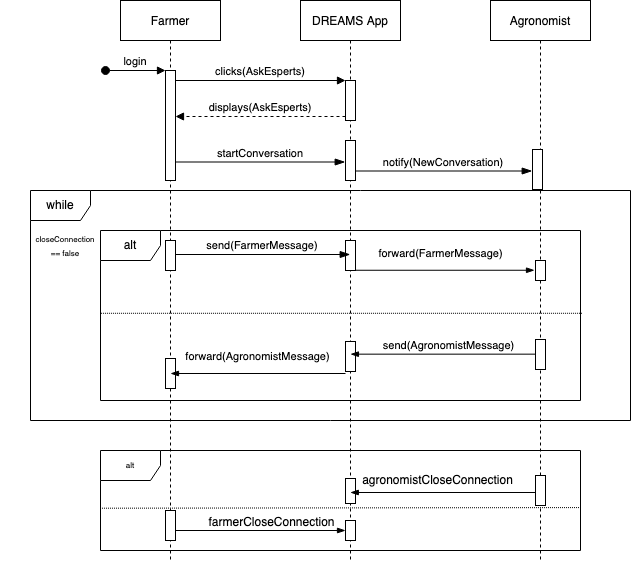
\includegraphics[scale=0.6]{Files/sequence_disgrams/thePNGs/farmer_askExperts.png}
\caption{\label{fig:farmerSeqRequest}Sequence Diagram for Farmer Requesting Help.}
\end{figure}

%
%\textbf{EXAMPLE:} if the system determines that precipitation levels are decreasing and enabling a water scarcity crisis, policy makers should be able to see that identify that trend in the system and this can motivate them to enforce policy such as investing in water irrigation technologies that increase efficiency and reduce water waste. Once such policies are in place, telengana policy makers can identify if the new policy mediates the water scarcity problem.
%\\
% Let's format the requirements table here in a seperate file. We will very likely modify the requirements later on so saving it in a seperate file might make it easier to: 1) see where we need to make modifications and 2) identify formatting errors.
\begin{center}
\begin{longtable}{|c|>{\raggedright\arraybackslash}m{15cm}|}

    \hline
    \multicolumn{2}{|c|}{Begin}\\\hline
    \textbf{ID} & \textbf{Requirement}\\\hline
    \endfirsthead
    
    \hline
    \multicolumn{2}{|c|}{Cont.}\\\hline
    \textbf{ID} & \textbf{Requirement}\\\hline
    \endhead 
 
 
R1	& The system must allow the farmer to set the production types of their fields.\\\hline
R2	& The system must allow the farmer to set the position of their fields manually.\\\hline
R3	& The system must allow the farmer to set the position of their fields through their devices' GPS.\\\hline
R4	& The system must keep track of the data about farmers.\\\hline
R5	& The system must provide an interface to visualize data.\\\hline
R6	& The system must be able to analyze data and show statistics.\\\hline
R7	& The system must enable farmers to modify their production type.\\\hline
R8	& The system must enable farmers to report issues they may face. \\\hline
R9	& The system must allow the farmer to report production data at a frequency chosen by the farmer. \\\hline
R10	& The system must retrieve the weather forecast data from the data that the Telengana government collects.\\\hline
R11	& The system must show updated weather forecast data at most 5 minutes from which the data has been published by the Telengana government.\\\hline
R12	& The system must provide weather data that forecasts at least 3 days ahead.\\\hline
R13	& The system must allow agronomists to access weather forecast data specific to their responsible area.\\\hline
R14	& The system must allow farmers to access weather forecast data based on their GPS location or from the location of their farm on record.\\\hline
R15	& The system must provide an interface for farmers to request help and suggestions from other farmers.\\\hline
R16	& The system must provide an interface for farmers to receive help requests and receive suggestions sent to them from other farmers.\\\hline
R17	& The system must provide an interface for farmers to provide suggestions to other farmers.\\\hline
R18	& The system must provide an interface for farmers to respond to help requests sent to them from other farmers.\\\hline
R19	& The system must provide an interface for farmers to request help and suggestions from other agronomists.\\\hline
R20	& The system must provide an interface for agronomists to receive help requests sent to them from other farmers.\\\hline
R21	& The system must provide an interface for agronomists to respond to help requests sent to them from other farmers.\\\hline
R22	& The system must provide an interface for agronomists to provide suggestions to other farmers.\\\hline
R23	& The system must provide a forum interface.\\\hline
R24	& The system must allow the farmer to create discussion forums.\\\hline
R25	& The system must allow farmers to view all posts in the discussion forum.\\\hline
R26	& The system must allow farmers to post replies in the discussion forum.\\\hline
R27	& The system must keep track of all the forum discussion.\\\hline
R28	& The system must allow agronomists to specify their responsible geographic area.\\\hline
R29	& The system must allow agronomists to modify their responsible geographic area.\\\hline 
R30	& The system must allow agronomist to view the list of all farmers in their area. \\\hline
R31	& The system must provide an evaluation of farmers such that the evaluation reflects the quality and quantity of their crop production.\\\hline
R32	& The system must enable agronomists to access farmer evaluations from their specific area.\\\hline
R33	& The system updates farmers' evaluation when new data is available.\\\hline % (ie, new farmer event entries or after an agronomist visit, etc)
R34	& The system must provide an interface for daily plans.\\\hline
R35	& The system must recommend which farmers should be included in the agronomist's daily plan.\\\hline
R36	& The system must generate recommendations such that farmers are visited by their respective agronomists at least twice a year.\\\hline
R37	& The system must generate recommendations such that farmers with low evaluation are visited more often than twice a year.\\\hline
R38	& The system must allow agronomist to view the list of all farms to visit on a specific day.\\\hline
R39	& The system must allow agronomists to modify which farmers they visit in their plan.\\\hline
R40	& The system must allow agronomists to specify and modify the duration of the visits in their plan.\\\hline
R41	& The system must maintain a record of farmers who have been visited by their respective agronomists.\\\hline
R42	& The system must allow agronomists to modify the daily plan at the end of the day.\\\hline
R43	& The system must allow agronomists to confirm that the daily plan was executed that the end of that day.\\\hline
R44	& The system must not allow anymore modifications to the plan after the plan is confirmed by the agronomist.\\\hline
R45	& The system must only generate a new plan for a new day after the plan from the preceding day was confirmed by the agronomist.\\\hline
R46	& The system must allow Telengana’s policy makers to view the list of all farmers.\\\hline
R47	& The system must allow Telengana’s policy makers to view the performance and evaluation of the farmers.\\\hline
R48	& The system must allow Telengana’s policy makers to view the ranking of the farmers.\\\hline
R49	& The system must allow Telengana’s policy makers to view well-performing and poor-performing farmers.\\\hline
R50	& The system must allow Telengana’s policy makers to flag the farmers that need to be helped based on their performance.\\\hline
R51	& The system must designate each farmer a measure of support received by agronomists and other well-performing farmers.\\\hline
R52	& The system must allow policy makers to view the history of farmers’ performance/ evaluation.\\\hline
R53	& The system must allow Telengana policy makers to view this measure of support designated to each farmer.\\\hline
\end{longtable}
\end{center}

% \input{Files/usecases/usecase6.tex}
% .......
\subsection{Goal mapping}
\newcommand\goal[1]{\item[[ G#1]]}
\newcommand\dom[1]{\item[[ D#1]]}
\newcommand\req[1]{\item[[ R#1]]}

Requirements must ensure satisfaction of the goal given the context of the domain assumption.


\begin{itemize}
\goal{1} \textbf{Farmers can visualize relevant data and suggestions based on their location and type of production.}

\begin{itemize}
\dom{1}  Users must have a device connected to internet.
\dom{2} To access to the system the user must have valid credentials.
\dom{3} The data about weather forecast, the farmers and their production, the sensors, the agronomist are correct, complete and sent to the application
\dom{4} The user has granted permission for GPS, notifications and disk usage
\dom{5} Farmers have an existing system to quantify, track, and organize their production yields
\dom{6} Users can successfully operate an interactive application

\req{1} The system must allow the farmer to set the production types of their fields.
\req{2} The system must allow the farmer to set the position of their fields manually.
\req{3} The system must allow the farmer to set the position of their fields through their devices' GPS.
\req{4} The system must keep track of the data about farmers
\req{5} The system must provide an interface to visualize data
\req{6} The system must be able to analyze data and show statistics
\req{7} The system must enable farmers to modify their production type.
\req{8} The system must enable farmers to report issues they may face. 
\req{9} The system must allow the farmer to report production data at a frequency chosen by the farmer.
\end{itemize}

\goal{2}  \textbf{Agronomists and farmers can view weather forecast data.}

\begin{itemize}
\dom{7} Business competition will not influence the farmers' willingness to help
\dom{8} Farmers are willing to ask for help from other farmers and/or agronomists
\dom{9} Farmers have industry knowledge about fertilizers, crops, etc 
\dom{10} Farmers are willing to interact with other farmers 

\req{10} The system must retrieve the weather forecast data from the data that the Telengana government collects.
\req{11} The system must show updated weather forecast data at most 5 minutes from which the data has been published by the Telengana government.
\req{12} The system must provide weather data that forecasts at least 3 days ahead
\req{13} The system must allow agronomists to access weather forecast data specific to their responsible area
\req{14} The system must allow farmers to access weather forecast data based on their GPS location [or from the location of thier farm on record]

\end{itemize}

\goal{3} \textbf{Farmers can interact with others farmers and agronomists by requesting for help and suggestions.}

\begin{itemize}


\req{15} The system must provide an interface for farmers to request help and suggestions from other farmers
\req{16} The system must provide an interface for farmers to recieve help requests and recieve suggestions sent to them from other farmers
\req{17} The system must provide an interface for farmers to provide suggestions to other farmers
\req{18} The system must provide an interface for farmers to respond to help requests sent to them from other farmers
\req{19} The system must provide an interface for farmers to request help and suggestions from other agronomists
\req{20} The system must provide an interface for agronomists to recieve help requests sent to them from other farmers
\req{21} The system must provide an interface for agronomists to respond to help requests sent to them from other farmers 
\req{22} The system must provide an interface for agronomists to provide suggestions to other farmers
\end{itemize}

\goal{4} \textbf{Farmers can create discussion forums with other farmers}
\begin{itemize}
\dom{11} Farmers can recognize issues and production abnormalities


\req{23}  The system must provide a forum interface
\req{24}  The system must allow the farmer to create discussion forums.
\req{25}  The system must allow the farmer to create discussion forums.
\req{26}  The system must allow farmers to post replies in the discussion forum
\req{27}  The system must keep track of all the forum discussion
\end{itemize}

\goal{5} \textbf{Agronomists can supervise a sub-area inside the region}
\begin{itemize}
\dom{12} Agronomists are assigned an area by their superiors
\dom{13} Agronomists can effectively manage an area assigned to them (ie, the agronomist is not overworked)

\req{28} The system must allow agronomists to specify the geographic area in which they are responsible for.
\req{29} The system must allow agronomists to specify the geographic area in which they are responsible for.
\end{itemize}

\goal{6} \textbf{Agronomists can view the ranking of farmers’ performance in their specific area.}
\begin{itemize}
\dom{14} Agronomists are experts in their field
\dom{15} Agronomists will be effective in addressing issues farmers face
\dom{15} DOMAIN ASSUMPTION RIPETUTAAAA (la 1)  Agronomists have access to an internet connection
\dom{16} DOMAIN ASSUMPTION RIPETUTAAAA (la 6)  Agronomists can successfully operate an interactive application

\req{30}  The system must be able to analyze data and show statistics
\req{31}  The system must allow agronomist to view the list of all farmers in their area.
\req{32}  The system must provide an evaluation of farmers such that the exaluation reflects the quality and quantity of their crop production
\req{33}  The system must enable agronomists to access farmer evaluations from their specific area
\req{34}  The system updates farmers' evaluation when new data is available (ie, new farmer event entries or after an agronomist visit, etc)
\end{itemize}

\goal{7} \textbf{Agronomists can visualize and update a daily plan to visit farms in their area}
\begin{itemize}



\req{35}  The system must provide an interface for daily plans
\req{36}  The system must recomend which farmers should be included in the agronomist's daily plan
\req{37}  The system must generate recomendations such that farmers are visited by their respective agronomists at least twice a year
\req{38}  The system must generate recomendations such that farmers with low evaluation are visited more often than twice a year
\req{39}  The system must allow agronomist to view the list of all farms to visit on a specific day.
\req{40}  The system must allow agronomists to modify which farmers they visit in their plan
\req{41}  The system must allow agronomists to specify and modify the duration of the visits in their plan
\req{42}  The system must maintain a record of farmers who have been visited by their respective agronomists

\end{itemize}

\goal{8} \textbf{Agronomists can specify the deviations from their daily plan and confirm the execution of their daily plan at the end of each day. }
\begin{itemize}
\req{43} The system must allow agronomists to modify the daily plan at the end of the day.
\req{44} The system must allow agronomists to confirm that the daily plan was executed that the end of that day
\req{45} The system must not allow anymore modifications to the plan after the plan is confirmed by the agronomist
\req{46} The system must only generate a new plan for a new day after the plan from the preceeding day was confirmed by the agronomist.
\end{itemize}

\goal{9} \textbf{Telengana’s policy makers can view the performance of the farmers and the ranking of the farmers. }
\begin{itemize}
\req{47} The system must allow Telengana’s policy makers to view the list of all farmers.
\req{48} The system must allow Telengana’s policy makers to view the performance and evaluation of the farmers.
\req{49} The system must allow Telengana’s policy makers to view the ranking of the farmers.
\req{50} The system must allow Telengana’s policy makers to view well-performing and poor-performing farmers.
\req{51} The system must allow Telengana’s policy makers to flag the farmers that need to be helped based on their performance.
\end{itemize}

\goal{10} \textbf{Telengana’s policy makers can use the system to determine if support from agronomists and well-performing farmers produces significant results.}

\begin{itemize}
\dom{24} Policy makers want to see the success of farmers in the form of production yields and crop quality

\req{52} The system must designate each farmer a measure of support received by agronomists and other well-performing farmers.
\req{53} The system must allow policy makers to view the history of farmers’ performance/ evaluation (score over time)
\req{54} The system must allow Telengana policy makers to view this measure of support designated to each farmer.
\end{itemize}



\end{itemize}


\subsubsection{Farmer}

\begin{flushleft}
The sequence diagram in \textbf{Figure \ref{fig:farmerSeqNewThread}} shows the exchange of information between the user and the DREAM application when the farmer user creates a new thread. After the user publishes the new thread, the DREAM application saves the submitted form and updates its servers.
\end{flushleft}

\begin{figure}[hbt!]
\centering
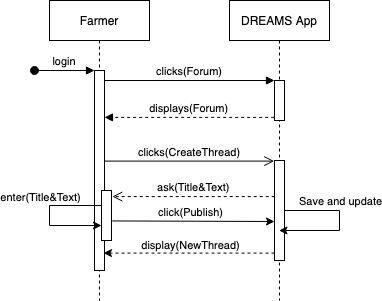
\includegraphics[scale=0.6]{Files/sequence_disgrams/thePNGs/farmer_createThread.png}\\
\caption{\label{fig:farmerSeqNewThread}Sequence Diagram for Farmer Creating Thread.}
\end{figure}


\begin{flushleft}
The sequence diagram in \textbf{Figure \ref{fig:farmerSeqNewField}} shows how the farmer user interacts with the DREAM application when adding a new field to their farm. Part of adding a new field to their farm involves providing the GPS location (if the user chooses to consent the DREAM application to access their location) and entering some information about the field such as the crop planted and the fertilizer used. After submitting the necessary information, the DREAM application saves and updated its servers and the farmer can then view the new field in their "My Farm" interface.
\end{flushleft}

\begin{figure}[htb!]
\centering
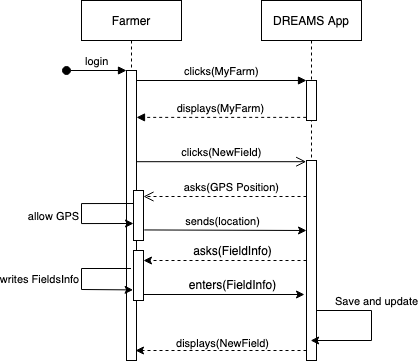
\includegraphics[scale=0.6]{Files/sequence_disgrams/thePNGs/farmer_newField.png}\\
\caption{\label{fig:farmerSeqNewField}Sequence Diagram for Farmer Adding Field.}
\end{figure}

\newpage
\subsubsection{Agronomist}

\begin{figure}[hpt!]
\centering
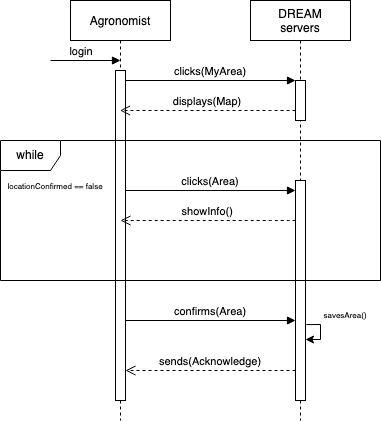
\includegraphics[scale=0.6]{Files/sequence_disgrams/thePNGs/agronomist_choosingLocation.png}\\
\caption{\label{fig:agrSeqArea}Sequence Diagram for Agronomist.}
\end{figure}

\begin{flushleft}
The sequence diagram in \textbf{Figure \ref{fig:agrSeqArea}} shows how the agronomist user interacts with the DREAM servers when modifying the area that they are responsible of with a map display interface.
\end{flushleft}


\begin{figure}[hpt!]
\centering
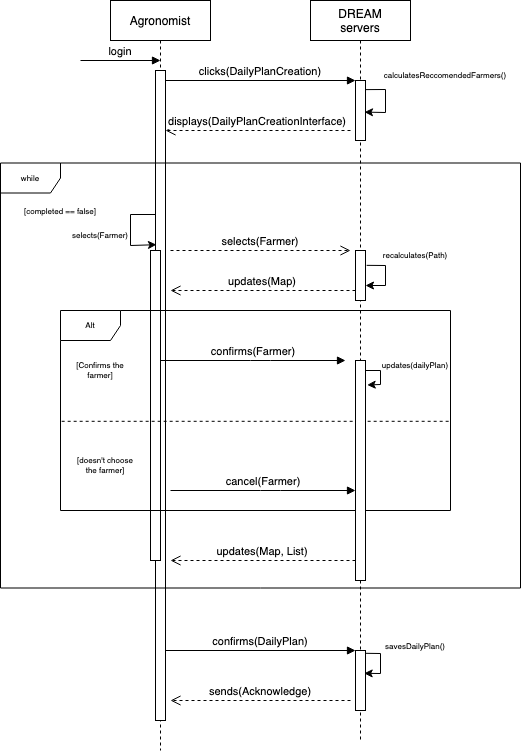
\includegraphics[scale=0.5]{Files/sequence_disgrams/thePNGs/agronomist_createPlan.png}\\
\caption{\label{fig:agrSeqCreatePlan}Sequence Diagram for Agronomist.}
\end{figure}
\begin{flushleft}
The sequence diagram in \textbf{Figure \ref{fig:agrSeqCreatePlan}}shows how the agronomist user interacts with the DREAM servers when creating a new daily plan in the daily plan interface including some of the specific calls that occur between the DREAM servers and the user's device. As the agronomist modifies the list of farmers to visit for the day, the agronomist's map is updated to show the new navigation path. From the list of farmers to visit, the agronomist can include or remove each farmer from the plan. Then, at the end, the agronomist can confirm the daily plan and the data is updated on the DREAM servers.
\end{flushleft}

\begin{figure}[hpt!]
\centering
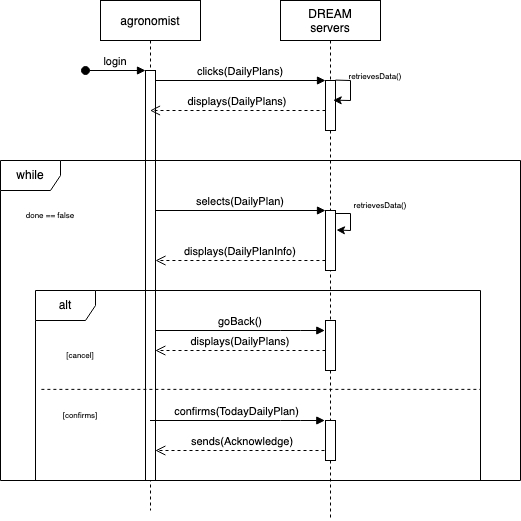
\includegraphics[scale=0.5]{Files/sequence_disgrams/thePNGs/agronomist_confirmPlan.png}\\
\caption{\label{fig:agrSeqConfirmPlan}Sequence Diagram for Agronomist.}
\end{figure}

\begin{flushleft}
At the end of a agronomist's day of visiting farmers, the agronomist has to confirm the execution of the plan. \textbf{Figure \ref{fig:agrSeqConfirmPlan}} shows how the agronomist user interacts with the DREAM servers when confirming a daily plan. Confirmation of a daily plan should occur after the agronomist has completed all the farmers they intend to visit that day. When confirming, the agronomist can modify the plan so that the plan accurately reflects the visits that the agronomist actually completed that day.
\end{flushleft}


\begin{figure}[hpt!]
\centering
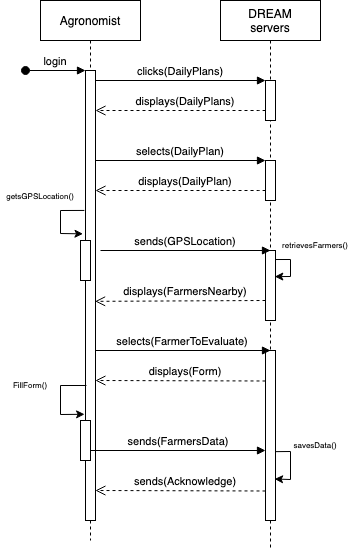
\includegraphics[scale=0.5]{Files/sequence_disgrams/thePNGs/agronomist_sendReport.png}\\
\caption{\label{fig:agrSeqSendReport}Sequence Diagram for Agronomist.}
\end{figure}

\begin{flushleft}
Thee sequence diagram in \textbf{Figure \ref{fig:agrSeqSendReport}} shows the interaction between the agronomist user and the DREAM servers when submitting a report evaluating the status of a farmer during a visit.
\end{flushleft}


\newpage
\subsubsection{Policy Maker}


\begin{flushleft}
The policy maker's use cases revolve around examining the results of the data analysis from a holistic point of view. The sequence diagram in \textbf{Figure \ref{fig:policySeqSetFlag}} shows how the policy maker user interacts with the DREAM servers when they set a flag on a farmer. After the policy maker flags a farmer from the ranking list view, the DREAM servers save the flag and send the policy maker user a confirmation that the flag has been set.
\end{flushleft}

\begin{figure}[hbt!]
\centering
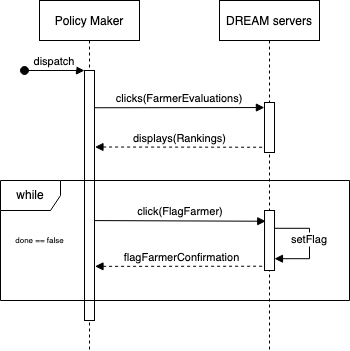
\includegraphics[scale=0.6]{Files/sequence_disgrams/thePNGs/policy_setFlag.png}\\
\caption{\label{fig:policySeqSetFlag}Sequence Diagram for Policy Maker.}
\end{figure}



\begin{flushleft}
The sequence diagram in \textbf{Figure \ref{fig:policySeqSetTrig}} shows how the policy maker user interacts with the DREAM servers when setting a trigger. Once the trigger parameters are set by the policy maker user, the DREAM servers saves them and confirms them with the user. Then, the data that the farmer enters thereafter is checked against the triggers saves on the DREAM servers. If the data entered satisfies a trigger, a notification is sent to the policy maker users.
\end{flushleft}

\begin{figure}[hbt!]
\centering
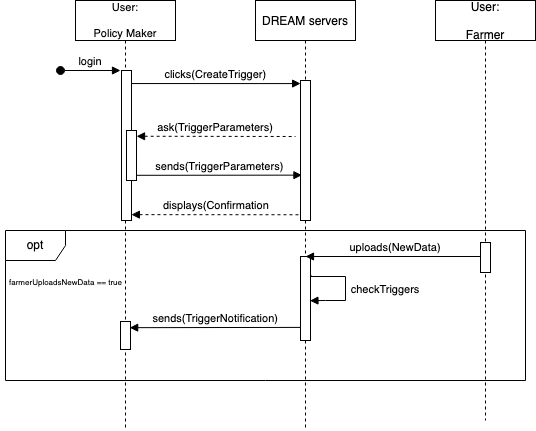
\includegraphics[scale=0.6]{Files/sequence_disgrams/thePNGs/policy_setTrigger.png}\\
\caption{\label{fig:policySeqSetTrig}Sequence Diagram for Policy Maker.}
\end{figure}


\begin{flushleft}
The sequence diagram in \textbf{Figure \ref{fig:policySeqViewRank}} shows the simple interaction between the policy maker user and the DREAM servers when the policy maker navigates to a ranking view. According to this sequence diagram, the ranking is calculated when the policy maker requests the view. This way, the view considers the most up-to-date data when ranking the farmers. The policy maker can also filter their view such as only considering corn farmers or only considering farmers from specific subareas.
\end{flushleft}

\begin{figure}[hbt!]
\centering
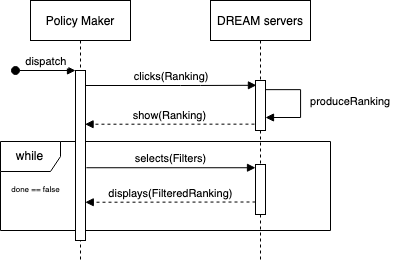
\includegraphics[scale=0.6]{Files/sequence_disgrams/thePNGs/policy_viewRanking.png}\\
\caption{\label{fig:policySeqViewRank}Sequence Diagram for Policy Maker.}
\end{figure}



\newpage
\subsection{Performance Requirements}

\begin{flushleft}

The DREAM application is expected to be accessed by users in the Telangana region. The servers should support over 1000 users simultaneously. The large majority of users will be farmers, whereas the number of policy makers and agronomists is strictly the number of government employees that anticipate utilizing DREAM as a tool to manage their job responsibilities. Farmers are expected to interact with the system while managing their fields in the day and agronomists and policy makers are expected to interact with the system strictly during business hours. From around 6:00 to 18:00 DREAM servers should sustain simultaneous requests from multiple users. Due to the large amount of data handled by the system it is crucial to ensure that data loss is minimal in order to preserve the integrity of the results of the data analysis produced by the system. For this reason, data integrity is prioritized over response time.\\
\end{flushleft}

\subsection{Design Constraints}


\subsubsection{Standards compliance}\label{standards}
DREAM application should be as safe and secure as possible: the users and their data must be protected.\\
The system should be compliant with the ISO/IEC 27001:2013 standard. This standard specifies the requirements for establishing, implementing, maintaining, and continually improving an information security management system within the context of the organization.
\subsubsection{Hardware limitations}

Since DREAM will be accessed from a mobile-friendly web application, there are few hardware limitations to consider. Instead, the limitations outlined will be easily met with common devices that are probably already used by the users.\smallskip\\
Policy makers already utilize a desktop computer for their work so with respect to the DREAM system they would need a screen that is large enough to comfortably view and configure the data visualizations offered by the DREAM application. Since DREAM will be accessed from a web application, the policy maker will need a modern internet browser; the operating system of the computer does not matter.\smallskip\\
Agronomists and farmers both may access the DREAM application from a mobile or tablet device. Current iOS/Android devices already come with GPS antennas, internet connectivity, and cameras, therefore no additional limitations need to be considered. Devices without a GPS antenna and without a camera can still be used to access the DREAM system but the user experience will be somewhat compromised: users will have to manually enter location information; users will not have turn-by-turn navigation guidance; and users will not be able to include pictures when describing issues or updates in their reports, forum posts, or help requests.\smallskip\\
Regarding the back-end, the system needs a server with constant internet access that can host the web application. A virtual machine on a cloud service, such as AWS or Azure, is a suitable solution to host the web application.\\

\subsubsection{Any other constraints}
\begin{flushleft}
Since users will have access to data visualizations, the interface should be simple enough as to no overwhelm the user but also ensure that the user has access to all the features, tools, and options when configuring their data views. Additionally, the format offered for farmers to report their data must be defined well enough so that DREAM can effectively parse through it and generate solutions with data analysis but also be flexible enough for farmers to capture qualitative data.
\end{flushleft}

\subsubsection{Reliability}
\begin{flushleft}
Since one of DREAM's primary value-add as a product is the data analysis, preserving the data is very important. In order to recover from potential data loss, offline data backups that are updated weekly are needed for redundancy. Ideally, the DREAM system should have the highest MTTF and the lowest MTTR as possible. However, since DREAM is not dealing with time-critical features, the system can afford a higher MTTR if pending data can be saved on the user's local device while waiting for DREAM system to recover.
\end{flushleft}

\subsubsection{Availability}
\begin{flushleft}

Since users depend on DREAM as a tool to execute their work, it is crucial to ensure the system is characterized by an availability of at least 99.9\%. This translates to about 10 minutes of downtime per week. This is tolerable because the system will be used primary during business hours and will have reduced usage or traffic during the weekends; policy makers and agronomists will likely not be accessing the DREAM application during the weekend but farmers might access the DREAM application.\smallskip\\
As mentioned, if users try to send data to the DREAM servers when they are unavailable, the data should get saved on the user's device until communication can be reestablished with the DREAM servers. Although this time duration may be perceivable to the end-user, the downtime does not interrupt the user experience since the system will handle the delayed communication. This mitigation technique ensures that the DREAM servers still receive all the data sent to it and the user's experience is not severely interrupted.\\ 
\end{flushleft}

\subsubsection{Security}
\begin{flushleft}
Government employees will be accessing the DREAM application with sensitive credentials. Additionally, the data produced by farmer users is associated with sensitive location data. The data around the daily plans for the agronomists contains location-identifying information during an agronomist's work day. Primarily due to these reasons, security should be prioritized in the design of the DREAM system to safeguard from data leaks, exploits, and malicious users.\smallskip\\
User credentials should be hashed and encrypted. Transactions, especially those involved with sensitive location data such as the daily plans or field GPS information, should only occur through connections that are secure and encrypted through the most updated version of TLS protocol. This minimizes the risk of data breaches.
\end{flushleft}

\subsubsection{Maintainability}
\begin{flushleft}
During the design, maintainability can only be sustained if good design, documentation, and coding practices are followed. Proper adherence to the standards cited in Section \ref{standards} will also preserve maintainability in the design of the system. Ensuring that the system is designed for maintainability will also enable the system to be easily scaleable; either to more farmers in the region, to other regions in India, or to other nations who wish to use DREAM.
\end{flushleft}

\subsubsection{Portability}
\begin{flushleft}
DREAM's web application should be compatible with a variety of operating systems, both mobile and non-mobile. Since DREAM is serving a market with a wide range of access to devices (from self-funded farmers to government-funded entities), DREAM system and layout should accommodate mobile users with a modern web browser, such as Chrome, Safari, or Firefox. Similarly, for users accessing DREAM from a computer, the OS must support a web browser, such as Chrome, Safari, or Firefox, in order to access the web application.
\end{flushleft}
